%%%%%%%%%%%%%%%%%%%%%%%%%%%%%%%%%%%%%%%%%
% Classicthesis Typographic Thesis
% LaTeX Template
% Version 1.4 (1/1/16)
%
% This template has been downloaded from:
% http://www.LaTeXTemplates.com
%
% Original author:
% André Miede (http://www.miede.de) with commenting modifications by:
% Vel (vel@LaTeXTemplates.com)
%
% License:
% GNU General Public License (v2)
%
% General Tips:
% 1) Make sure to edit the classicthesis-config.file
% 2) New enumeration (A., B., C., etc in small caps): \begin{aenumerate} \end{aenumerate}
% 3) For margin notes: \marginpar or \graffito{}
% 4) Do not use bold fonts in this style, it is designed around them
% 5) Use tables as in the examples
% 6) See classicthesis-preamble.sty for useful commands
%
%%%%%%%%%%%%%%%%%%%%%%%%%%%%%%%%%%%%%%%%%

%----------------------------------------------------------------------------------------
%	PACKAGES AND OTHER DOCUMENT CONFIGURATIONS
%----------------------------------------------------------------------------------------

\documentclass[
		twoside,openright,titlepage,numbers=noenddot,headinclude,justified,%1headlines,
	 	footinclude=true,cleardoublepage=empty,
		dottedtoc, % Make page numbers in the table of contents flushed right with dots leading to them
    BCOR=10mm,paper=a4,fontsize=11pt, % Binding correction, paper type and font size
    % footheight=52pt,
    ngerman,american, % Languages, change this to your language(s)
		]{scrreprt} %tufte-book  scrreprt

% Includes the file which contains all the document configurations and packages - make sure to edit this file
%%%%%%%%%%%%%%%%%%%%%%%%%%%%%%%%%%%%%%%%%
% Classicthesis Typographic Thesis
% Configuration File
%
% This file has been downloaded from:
% http://www.LaTeXTemplates.com
%
% Original author:
% André Miede (http://www.miede.de) with extensive commenting changes by:
% Vel (vel@LaTeXTemplates.com)
%
% License:
% GNU General Public License (v2)
%
% Important note:
% The main lines to change in this file are in the DOCUMENT VARIABLES
% section, the rest of the file is for advanced configuration.
%
%%%%%%%%%%%%%%%%%%%%%%%%%%%%%%%%%%%%%%%%%

%----------------------------------------------------------------------------------------
%	CHARACTER ENCODING
%----------------------------------------------------------------------------------------

\PassOptionsToPackage{utf8}{inputenc} % Set the encoding of your files. UTF-8 is the only sensible encoding nowadays. If you can't read äöüßáéçèê∂åëæƒÏ€ then change the encoding setting in your editor, not the line below. If your editor does not support utf8 use another editor!
\usepackage{inputenc}

%----------------------------------------------------------------------------------------
%	DOCUMENT VARIABLES
%	Fill in the lines below to enter your information into the thesis template
%	Each of the commands can be cited anywhere in the thesis
%----------------------------------------------------------------------------------------

% Remove drafting to get rid of the '[ Date - classicthesis version 4.0 ]' text at the bottom of every page
\PassOptionsToPackage{eulerchapternumbers,listings,drafting, pdfspacing, subfig,beramono,eulermath,parts}{classicthesis}
% Available options: drafting parts nochapters linedheaders eulerchapternumbers beramono eulermath pdfspacing minionprospacing tocaligned dottedtoc manychapters listings floatperchapter subfig

% \newcommand{\myTitle}{Investigating electron identification and energy regression
%                       in the forward region in ATLAS\xspace}
\newcommand{\myTitle}{\fontfamily{lmr}\selectfont 
                      TITLE \xspace %% Adjust vspace according to the title length.
                     }
\newcommand{\mySubtitle}{\xspace}
\newcommand{\myDegree}{Master of Science (Cand.scient.)\xspace}
\newcommand{\myName}{Your name\xspace}
\newcommand{\myMail}{Your mail\xspace}
\newcommand{\myProf}{Put name here\xspace} % I didnt use this
\newcommand{\myOtherProf}{Put name here\xspace} % I didnt use this
\newcommand{\mySupervisor}{Supervisor name\xspace}
\newcommand{\mySupervisorMail}{Supervisor mail\xspace}
\newcommand{\myFaculty}{Faculty of Science\xspace}
\newcommand{\myDepartment}{Niels Bohr Institute\xspace}
\newcommand{\myUni}{University of Copenhagen\xspace}
\newcommand{\myLocation}{Copenhagen\xspace}
\newcommand{\myTime}{7\ts{th} of Spooktober, 2020\xspace} %September 2015
\newcommand{\myVersion}{version 1.0\xspace}

%----------------------------------------------------------------------------------------
%	USEFUL COMMANDS
%----------------------------------------------------------------------------------------

\newcommand{\ie}{i.\,e.}
\newcommand{\Ie}{I.\,e.}
\newcommand{\eg}{e.\,g.}
\newcommand{\Eg}{E.\,g.}

\newcommand{\ts}{\textsuperscript}

\newcounter{dummy} % Necessary for correct hyperlinks (to index, bib, etc.)
\providecommand{\mLyX}{L\kern-.1667em\lower.25em\hbox{Y}\kern-.125emX\@}
\newlength{\abcd} % for ab..z string length calculation

%----------------------------------------------------------------------------------------
%	PACKAGES
%----------------------------------------------------------------------------------------

\usepackage{lipsum} % Used for inserting dummy 'Lorem ipsum' text into the template

%------------------------------------------------

%\PassOptionsToPackage{ngerman,american}{babel}  % Change this to your language(s)
% Spanish languages need extra options in order to work with this template
%\PassOptionsToPackage{spanish,es-lcroman}{babel}
\usepackage{babel}

%------------------------------------------------			

\usepackage{csquotes}
\PassOptionsToPackage{%
%backend=biber, % Instead of bibtex
backend=bibtex8,bibencoding=ascii,%
language=auto,%
style=numeric-comp,%
%style=authoryear-comp, % Author 1999, 2010
%bibstyle=authoryear,dashed=false, % dashed: substitute rep. author with ---
sorting=nyt, % name, year, title
maxbibnames=10, % default: 3, et al.
%backref=true,%
natbib=true % natbib compatibility mode (\citep and \citet still work)
}{biblatex}
\usepackage{biblatex}
 
 %------------------------------------------------

\PassOptionsToPackage{fleqn}{amsmath} % Math environments and more by the AMS 
 \usepackage{amsmath}
 
 %------------------------------------------------

\PassOptionsToPackage{T1}{fontenc} % T2A for cyrillics
\usepackage{fontenc}

%------------------------------------------------

\usepackage{textcomp} % Fix warning with missing font shapes

%------------------------------------------------

\usepackage{scrhack} % Fix warnings when using KOMA with listings package  

%------------------------------------------------

\usepackage{xspace} % To get the spacing after macros right

%------------------------------------------------

\usepackage{mparhack} % To get marginpar right

%------------------------------------------------

\usepackage{fixltx2e} % Fixes some LaTeX stuff 

%------------------------------------------------

% \PassOptionsToPackage{smaller,withpage}{acronym} % Include printonlyused in the first bracket to only show acronyms used in the text
\usepackage[smaller,withpage]{acronym} % Nice macros for handling all acronyms in the thesis

%\renewcommand*{\acsfont}[1]{\textssc{#1}} % For MinionPro
\renewcommand*{\aclabelfont}[1]{\acsfont{#1}}

%------------------------------------------------

\PassOptionsToPackage{pdftex}{graphicx}
\usepackage{xcolor} % \color{red} to color text
\usepackage{graphicx} % \includegraphics
\usepackage{eso-pic} % \AddToShipoutPicture
\usepackage{hyperref} % Link refferences \href
\usepackage{tcolorbox} % \begin{tcolorbox}  for textboxes
% \usepackage{tufte-sidenotes} % \sidenote{}
\usepackage{sidenotes}
\usepackage{hyperref}
\usepackage{gensymb}
\usepackage{varwidth}
\usepackage{marginnote}
\usepackage{nccmath}
\usepackage{makecell}
\usepackage{braket}
\usepackage{subfig}
\usepackage{slashed}
\usepackage{multirow}
\usepackage{array}
\usepackage{float}
% \usepackage[top=3in]{geometry}

% \usepackage{perpage} %the perpage package
% \MakePerPage{footnote} %the perpage package command
\usepackage[stable, perpage]{footmisc} %,side

\newcommand{\marnote}[1] { \marginnote{\begin{footnotesize} #1 \end{footnotesize}} }
%----------------------------------------------------------------------------------------
%	FLOATS: TABLES, FIGURES AND CAPTIONS SETUP
%----------------------------------------------------------------------------------------

\usepackage{tabularx} % Better tables
\setlength{\extrarowheight}{3pt} % Increase table row height
\newcommand{\tableheadline}[1]{\multicolumn{1}{c}{\spacedlowsmallcaps{#1}}}
\newcommand{\myfloatalign}{\centering} % To be used with each float for alignment
\usepackage{caption}
\captionsetup{font=small}
\usepackage{subfig}  

%----------------------------------------------------------------------------------------
%	CODE LISTINGS SETUP
%----------------------------------------------------------------------------------------

\usepackage{listings} 
%\lstset{emph={trueIndex,root},emphstyle=\color{BlueViolet}}%\underbar} % For special keywords
\lstset{language=[LaTeX]Tex,%C++ % Specify the language(s) for listings here
morekeywords={PassOptionsToPackage,selectlanguage},
keywordstyle=\color{RoyalBlue}, % Add \bfseries for bold  %%Was RoyalBlue
basicstyle=\small\ttfamily, % Makes listings a smaller font size and a different font
%identifierstyle=\color{NavyBlue}, % Color of text inside brackets
commentstyle=\color{Green}\ttfamily, % Color of comments
stringstyle=\rmfamily, % Font type to use for strings
numbers=left, % Change left to none to remove line numbers
numberstyle=\scriptsize, % Font size of the line numbers
stepnumber=5, % Increment of line numbers
numbersep=8pt, % Distance of line numbers from code listing
showstringspaces=false, % Sets whether spaces in strings should appear underlined
breaklines=true, % Force the code to stay in the confines of the listing box
%frameround=ftff, % Uncomment for rounded frame
%frame=single, % Frame border - none/leftline/topline/bottomline/lines/single/shadowbox/L
belowcaptionskip=.75\baselineskip % Space after the "Listing #: Desciption" text and the listing box
}

%----------------------------------------------------------------------------------------
%	HYPERREFERENCES
%----------------------------------------------------------------------------------------

\PassOptionsToPackage{pdftex,pdfpagelabels}{hyperref} %hyperfootnotes=false,
\usepackage{hyperref}  % backref linktocpage pagebackref
\pdfcompresslevel=9
\pdfadjustspacing=1

\hypersetup{
% Uncomment the line below to remove all links (to references, figures, tables, etc), useful for b/w printouts
%draft, 
colorlinks=true, linktocpage=true, pdfstartpage=3, pdfstartview=FitV,
% Uncomment the line below if you want to have black links (e.g. for printing black and white)
%colorlinks=false, linktocpage=false, pdfborder={0 0 0}, pdfstartpage=3, pdfstartview=FitV, 
breaklinks=true, pdfpagemode=UseNone, pageanchor=true, pdfpagemode=UseOutlines,%
plainpages=false, bookmarksnumbered, bookmarksopen=true, bookmarksopenlevel=1,%
hypertexnames=true, pdfhighlight=/O,%nesting=true,%frenchlinks,%
urlcolor=webbrown, linkcolor=RoyalBlue, citecolor=webgreen, %pagecolor=RoyalBlue,%
    %urlcolor=Black, linkcolor=Black, citecolor=Black, %pagecolor=Black,%
%------------------------------------------------
% PDF file meta-information
pdftitle={\myTitle},
pdfauthor={\textcopyright\ \myName, \myUni, \myFaculty},
pdfsubject={},
pdfkeywords={},
pdfcreator={pdfLaTeX},
pdfproducer={LaTeX with hyperref and classicthesis}
%------------------------------------------------
}

%----------------------------------------------------------------------------------------
%	AUTOREFERENCES SETUP
%	Redefines how references in text are prefaced for different 
%	languages (e.g. "Section 1.2" or "section 1.2")
%----------------------------------------------------------------------------------------

\makeatletter
\@ifpackageloaded{babel}
{
\addto\extrasamerican{
\renewcommand*{\figureautorefname}{Figure}
\renewcommand*{\tableautorefname}{Table}
\renewcommand*{\partautorefname}{Part}
\renewcommand*{\chapterautorefname}{Chapter}
\renewcommand*{\sectionautorefname}{Section}
\renewcommand*{\subsectionautorefname}{Section}
\renewcommand*{\subsubsectionautorefname}{Section}
}
\addto\extrasngerman{
\renewcommand*{\paragraphautorefname}{Absatz}
\renewcommand*{\subparagraphautorefname}{Unterabsatz}
\renewcommand*{\footnoteautorefname}{Fu\"snote}
\renewcommand*{\FancyVerbLineautorefname}{Zeile}
\renewcommand*{\theoremautorefname}{Theorem}
\renewcommand*{\appendixautorefname}{Anhang}
\renewcommand*{\equationautorefname}{Gleichung}
\renewcommand*{\itemautorefname}{Punkt}
}
\providecommand{\subfigureautorefname}{\figureautorefname} % Fix to getting autorefs for subfigures right
}{\relax}
\makeatother

%----------------------------------------------------------------------------------------

\usepackage{classicthesis} 

%----------------------------------------------------------------------------------------
%	CHANGING TEXT AREA 
%----------------------------------------------------------------------------------------

%\linespread{1.05} % a bit more for Palatino
%\areaset[current]{312pt}{761pt} % 686 (factor 2.2) + 33 head + 42 head \the\footskip
%\setlength{\marginparwidth}{7em}%
%\setlength{\marginparsep}{2em}%
\addtolength{\topmargin}{10pt} %std: 10pt -> 12pt
\addtolength{\headsep}{23pt} %std: 25pt

%----------------------------------------------------------------------------------------
%	USING DIFFERENT FONTS
%----------------------------------------------------------------------------------------

%\usepackage[oldstylenums]{kpfonts} % oldstyle notextcomp
%\usepackage[osf]{libertine}
%\usepackage[light,condensed,math]{iwona}
%\renewcommand{\sfdefault}{iwona}
%\usepackage{lmodern} % <-- no osf support :-(
%\usepackage{cfr-lm} % 
%\usepackage[urw-garamond]{mathdesign} <-- no osf support :-(
%\usepackage[default,osfigures]{opensans} % scale=0.95 
%\usepackage[sfdefault]{FiraSans}

%----------------------------------------------------------------------------------------
%	SET UP CAPTION SETTINGS
%----------------------------------------------------------------------------------------

\definecolor{nice_red_mahdude}{RGB}{173,49,54}

\captionsetup{
justification=raggedright,
labelfont={color=nice_red_mahdude,bf}, font=footnotesize,
%font=small,textfont=it,
indention=0pt,format=plain}

%----------------------------------------------------------------------------------------
%	SET COLORS
%----------------------------------------------------------------------------------------



\addbibresource{Bibliography.bib} % The file housing your bibliography
%\addbibresource[label=ownpubs]{Self_Publications.bib} % Uncomment for optional self-publications
  
%\hyphenation{Put special hyphenation here}

% Being centering
\def \ColourPDF {FrontBackMatter/ku-farve.pdf}
\def \TitlePDF   {FrontBackMatter/nat-en.pdf}
\title{
  % \vspace{-1cm}
  \normalsize{A thesis presented to the Faculty of Science} \\
  \large{Master of Science in physics at the Niels Bohr Institute} \\
  \vspace{1cm}
  \centering
  \Huge{\vspace{2cm} \myTitle}\\ %Ajdust vspace according to title length.
  % \huge{\mySubtitle}\\
}
\author{
  \huge{\myName} \\
  \normalsize{\texttt{\myMail}}
  \vspace{7cm} \\
  \large{\mySupervisor} \\
  \normalsize{\texttt{\mySupervisorMail}} \\
  \vspace{1cm} \\
}
\date{\myTime}
 
\begin{document}
\addtolength{\topmargin}{12pt}

\frenchspacing % Reduces space after periods to make text more compact

\raggedbottom % Makes all pages the height of the text on that page

\selectlanguage{american} % Select your default language - e.g. american or ngerman

%\renewcommand*{\bibname}{new name} % Uncomment to change the name of the bibliography
%\setbibpreamble{} % Uncomment to include a preamble to the bibliography - some text before the reference list starts

\pagenumbering{roman} % Roman page numbering prior to the start of the thesis content (i, ii, iii, etc)

\pagestyle{plain} % Suppress headers for the pre-content pages

%----------------------------------------------------------------------------------------
%	PRE-CONTENT THESIS PAGES
%----------------------------------------------------------------------------------------

\AddToShipoutPicture*{\put(0,0){\includegraphics*[viewport=0 0 700 600]{\ColourPDF}}}
\AddToShipoutPicture*{\put(0,602){\includegraphics*[viewport=0 600 700 1600]{\ColourPDF}}}
\AddToShipoutPicture*{\put(0,0){\includegraphics*{\TitlePDF}}}

\maketitle

% Back of the title page

\thispagestyle{empty}

\hfill

\vfill

\noindent\myName: \textit{\myTitle,} \myDegree, 
\textcopyright\ \myTime

% You may wish to do something with the back of the title page, such as including your supervisors, location or time frame of the work. Below is an example of doing so although you may want to tweak it to your liking.

%\bigskip

%\noindent\spacedlowsmallcaps{Supervisors}: \\
%\myProf \\
%\myOtherProf \\ 
%\mySupervisor

%\medskip \\

%\noindent\spacedlowsmallcaps{Location}: \\
%\myLocation

%\medskip \\

%\noindent\spacedlowsmallcaps{Time Frame}: \\
%\myTime
 % Back of the title page

% \cleardoublepage% Dedication

\thispagestyle{empty}
\refstepcounter{dummy}

\pdfbookmark[1]{Dedication}{Dedication} % Bookmark name visible in a PDF viewer

\vspace*{3cm}

\begin{center}
\emph{Ohana} means family. \\
Family means nobody gets left behind, or forgotten. \\ \medskip
--- Lilo \& Stitch    
\end{center}

\medskip

\begin{center}
Dedicated to the loving memory of Rudolf Miede. \\ \smallskip
1939\,--\,2005
\end{center} % Uncomment and create a Dedication.tex to include a dedication

%\cleardoublepage\include{FrontBackMatter/Foreword} % Uncomment and create a Foreword.tex to include a foreword

\cleardoublepage% Abstract

%\renewcommand{\abstractname}{Abstract} % Uncomment to change the name of the abstract

\pdfbookmark[1]{Abstract}{Abstract} % Bookmark name visible in a PDF viewer

\begingroup
\let\clearpage\relax
\let\cleardoublepage\relax
\let\cleardoublepage\relax

\chapter*{Abstract}
%% State the problem
\noindent THE ABSTRACT

% Colorcoding for thesis: \\
% \color{red} Things for hard review/rewriting! \\
% \color{blue} Things that need rewording \\
% \color{yellow} Things that perhaps need to be deleted \\
% \color{green} Things that need to be expanded upon \\
% \color{orange} Needs to be fact checked \\


\endgroup			

\vfill % Abstract page

% \cleardoublepage\include{FrontBackMatter/Publications} % Publications from the thesis page

\cleardoublepage% Acknowledgements

\pdfbookmark[1]{Acknowledgements}{Acknowledgements} % Bookmark name visible in a PDF viewer

% \begin{flushright}{\slshape    
% 'Tis better to have coded and debugged than never to have coded at all.} \\ \medskip
% --- Loui Wentzel
% \end{flushright}

\bigskip

%----------------------------------------------------------------------------------------

\begingroup

\let\clearpage\relax
\let\cleardoublepage\relax
\let\cleardoublepage\relax

\chapter*{Acknowledgements}

\noindent I Acknowledge myself. \\
Good job me.


\endgroup % Acknowledgements page

\cleardoublepage% Acknowledgements

\pdfbookmark[1]{Introduction}{Introduction} % Bookmark name visible in a PDF viewer

\begingroup

\let\clearpage\relax
\let\cleardoublepage\relax
\let\cleardoublepage\relax

\chapter*{Introduction}

\noindent *INtro*

\endgroup


 % Publications from the thesis page

\pagestyle{scrheadings} % Show chapter titles as headings

\cleardoublepage% Table of Contents - List of Tables/Figures/Listings and Acronyms

\refstepcounter{dummy}

\pdfbookmark[1]{\contentsname}{tableofcontents} % Bookmark name visible in a PDF viewer

\setcounter{tocdepth}{2} % Depth of sections to include in the table of contents - currently up to subsections

\setcounter{secnumdepth}{3} % Depth of sections to number in the text itself - currently up to subsubsections

\manualmark
\markboth{\spacedlowsmallcaps{\contentsname}}{\spacedlowsmallcaps{\contentsname}}
\tableofcontents 
\automark[section]{chapter}
\renewcommand{\chaptermark}[1]{\markboth{\spacedlowsmallcaps{#1}}{\spacedlowsmallcaps{#1}}}
\renewcommand{\sectionmark}[1]{\markright{\thesection\enspace\spacedlowsmallcaps{#1}}}

\clearpage

% \begingroup 
% \let\clearpage\relax
% \let\cleardoublepage\relax
% \let\cleardoublepage\relax

% %----------------------------------------------------------------------------------------
% %	List of Figures
% %----------------------------------------------------------------------------------------

% \refstepcounter{dummy}
% %\addcontentsline{toc}{chapter}{\listfigurename} % Uncomment if you would like the list of figures to appear in the table of contents
% \pdfbookmark[1]{\listfigurename}{lof} % Bookmark name visible in a PDF viewer

% \listoffigures

% \vspace{8ex}
% \newpage

% %----------------------------------------------------------------------------------------
% %	List of Tables
% %----------------------------------------------------------------------------------------

% \refstepcounter{dummy}
% %\addcontentsline{toc}{chapter}{\listtablename} % Uncomment if you would like the list of tables to appear in the table of contents
% \pdfbookmark[1]{\listtablename}{lot} % Bookmark name visible in a PDF viewer

% \listoftables
        
% \vspace{8ex}
% \newpage
    
% % %----------------------------------------------------------------------------------------
% % %	List of Listings
% % %---------------------------------------------------------------------------------------- 

% % \refstepcounter{dummy}
% % %\addcontentsline{toc}{chapter}{\lstlistlistingname} % Uncomment if you would like the list of listings to appear in the table of contents
% % \pdfbookmark[1]{\lstlistlistingname}{lol} % Bookmark name visible in a PDF viewer

% % \lstlistoflistings 

% % \vspace{8ex}
% % \newpage
       
% % %----------------------------------------------------------------------------------------
% % %	Acronyms
% % %----------------------------------------------------------------------------------------

% % \refstepcounter{dummy}
% % %\addcontentsline{toc}{chapter}{Acronyms} % Uncomment if you would like the acronyms to appear in the table of contents
% % \pdfbookmark[1]{Acronyms}{acronyms} % Bookmark name visible in a PDF viewer

% % \markboth{\spacedlowsmallcaps{Acronyms}}{\spacedlowsmallcaps{Acronyms}}

% % \chapter*{Acronyms}

% % \begin{acronym}[UML]
% % \acro{DRY}{Don't Repeat Yourself}
% % \acro{API}{Application Programming Interface}
% % \acro{UML}{Unified Modeling Language}
% % \end{acronym}  
                   
% \endgroup % Contents, list of figures/tables/listings and acronyms

\cleardoublepage

\pagenumbering{arabic} % Arabic page numbering for thesis content (1, 2, 3, etc)
%\setcounter{page}{90} % Uncomment to manually start the page counter at an arbitrary value (for example if you wish to count the pre-content pages in the page count)

\cleardoublepage % Avoids problems with pdfbookmark

%----------------------------------------------------------------------------------------
%	THESIS CONTENT - CHAPTERS
%----------------------------------------------------------------------------------------

\part{The Lord of the Rings}

\chapter{The Fellowship of the ring}
\label{ch:fellowship} % For referencing the chapter elsewhere, use \autoref{ch:introduction} 
\begin{tcolorbox}
  I am a pretext!
\end{tcolorbox}

\section{The Shire} \label{sec:shire}
I will site a book!
\citetitle{srednicki:2006} by \citeauthor{srednicki:2006} \citep{srednicki:2006}.
\begin{figure}
  \marginnote{
  \caption{Simple overview of the elementary particles of the Standard Model.
  Schematic from \citeauthor{Purcell:2012} \citep{Purcell:2012}}
  \label{fig:SMinfographic}}
  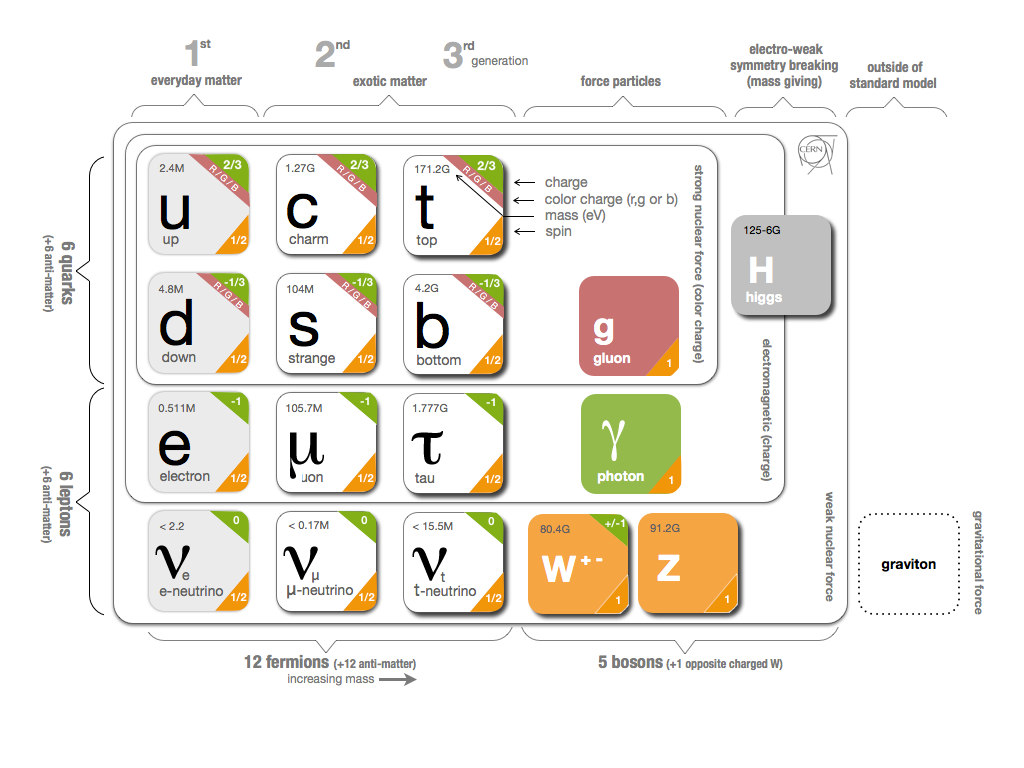
\includegraphics[width=1.15\linewidth]{Images/Part_1/SMinfographic_image.png}
\end{figure}

\subsection{Frodo be chillin} \label{sec:frodoNchill}
Not a lot happens

\subsection{Gandalf Commth} \label{sec:bitchImGandalf}
Some weird shit happens
Here's a figure on the side! Use Hspace and Vspace to fineadjust.


\chapter{The Two Towers} \label{ch:towers}
In \autoref{ch:fellowship} we see that pippin is pimpin.
The first chapter has the label 'ch:fellowship'.
Using ref gives: \ref{ch:fellowship}. Using autoref gives: \autoref{ch:fellowship}.
\marginnote{
    \hspace*{-0.5cm}
    \vspace*{0.5cm}
    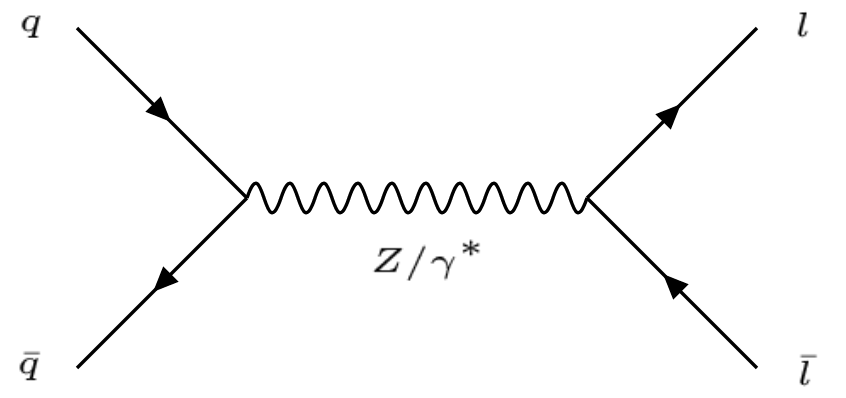
\includegraphics[width=1.6\marginparwidth]{Images/Part_1/MainDecayPath.png}
    \captionof{figure}{Feynman diagram for the $q\bar{q} \rightarrow Z/\gamma^* \rightarrow l\bar{l}$ decay where $\gamma^*$ is a virtual photon}
    \label{fig:MainDecay}
}

\subsection{Feynman diagrams} \label{sec:Feynman}
We are not only interested in the probability of collision, but also how particles in that collision decays
and what they decay to after an interaction.
This requires some theoretical calculation. Fermi's Golden rule describes the probability of some initial particle (\textit{i}) decaying
into a specific final mode \textit{f} and is given by \citep{schwartz:2006}:
\begin{ceqn}\begin{align} \label{eq:adamisgay}
  \centering
  \Gamma_{i \rightarrow f} \sim |M_{i \rightarrow f}|^2 \delta(E_f-E_i)
\end{align}\end{ceqn}
\autoref{eq:adamisgay} is an equation.

\chapter{The Return of the King} \label{ch:king}
The best one \\

An acronym the first time it is used: \ac{CERN}.\\
An acronym the post-first time: \ac{CERN}

\cleardoublepage

%------------------------------------------------

\part{The Hobbit} 

\chapter{Let's waste 10 hours in the shire - the movie}
AAAAAAAAAAAAAAAAAAAAAAAAAAAAAAAAAAAAAAAAAAAAAAAAA

\begin{figure}
  \marginnote{
  \caption{A very cute cat}}
  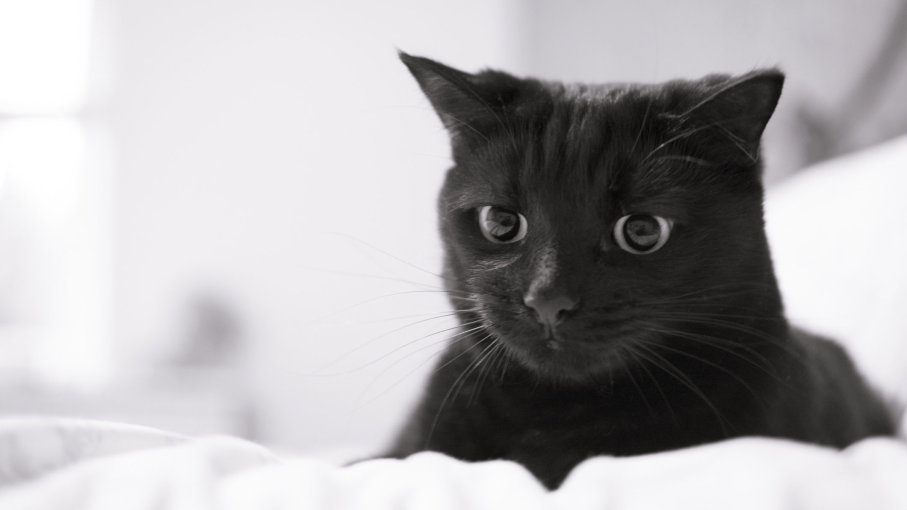
\includegraphics[width=1\linewidth]{Images/tesla-cat.jpg}
\end{figure}

\chapter{Some shit or something idk don't rember}

\section{blop}

\section{Same blop}

\chapter{Wait there's three?}

\cleardoublepage

%------------------------------------------------

% \part{Name of chapter in document} 

% \include{name of chapter file}

% \cleardoublepage % Empty page before the start of the next part

%----------------------------------------------------------------------------------------
%	THESIS CONTENT - APPENDICES
%----------------------------------------------------------------------------------------

\appendix

\part{Appendices} % Appendicies

%% You can add more appendicies
% Appendix A

\chapter{Appendix A: Theory and production} \label{App:A:} 

\begin{figure}
  \vspace*{-0.5cm}
  \marginnote{
      \caption{A comparison of two different targets when training a regression model.
      Top graph showing the true energy as target. Bottom graph showing the true energy 
      divided by the raw E Cluster energy measured by the detector}
      \label{fig:ER_taget_comparison}}
  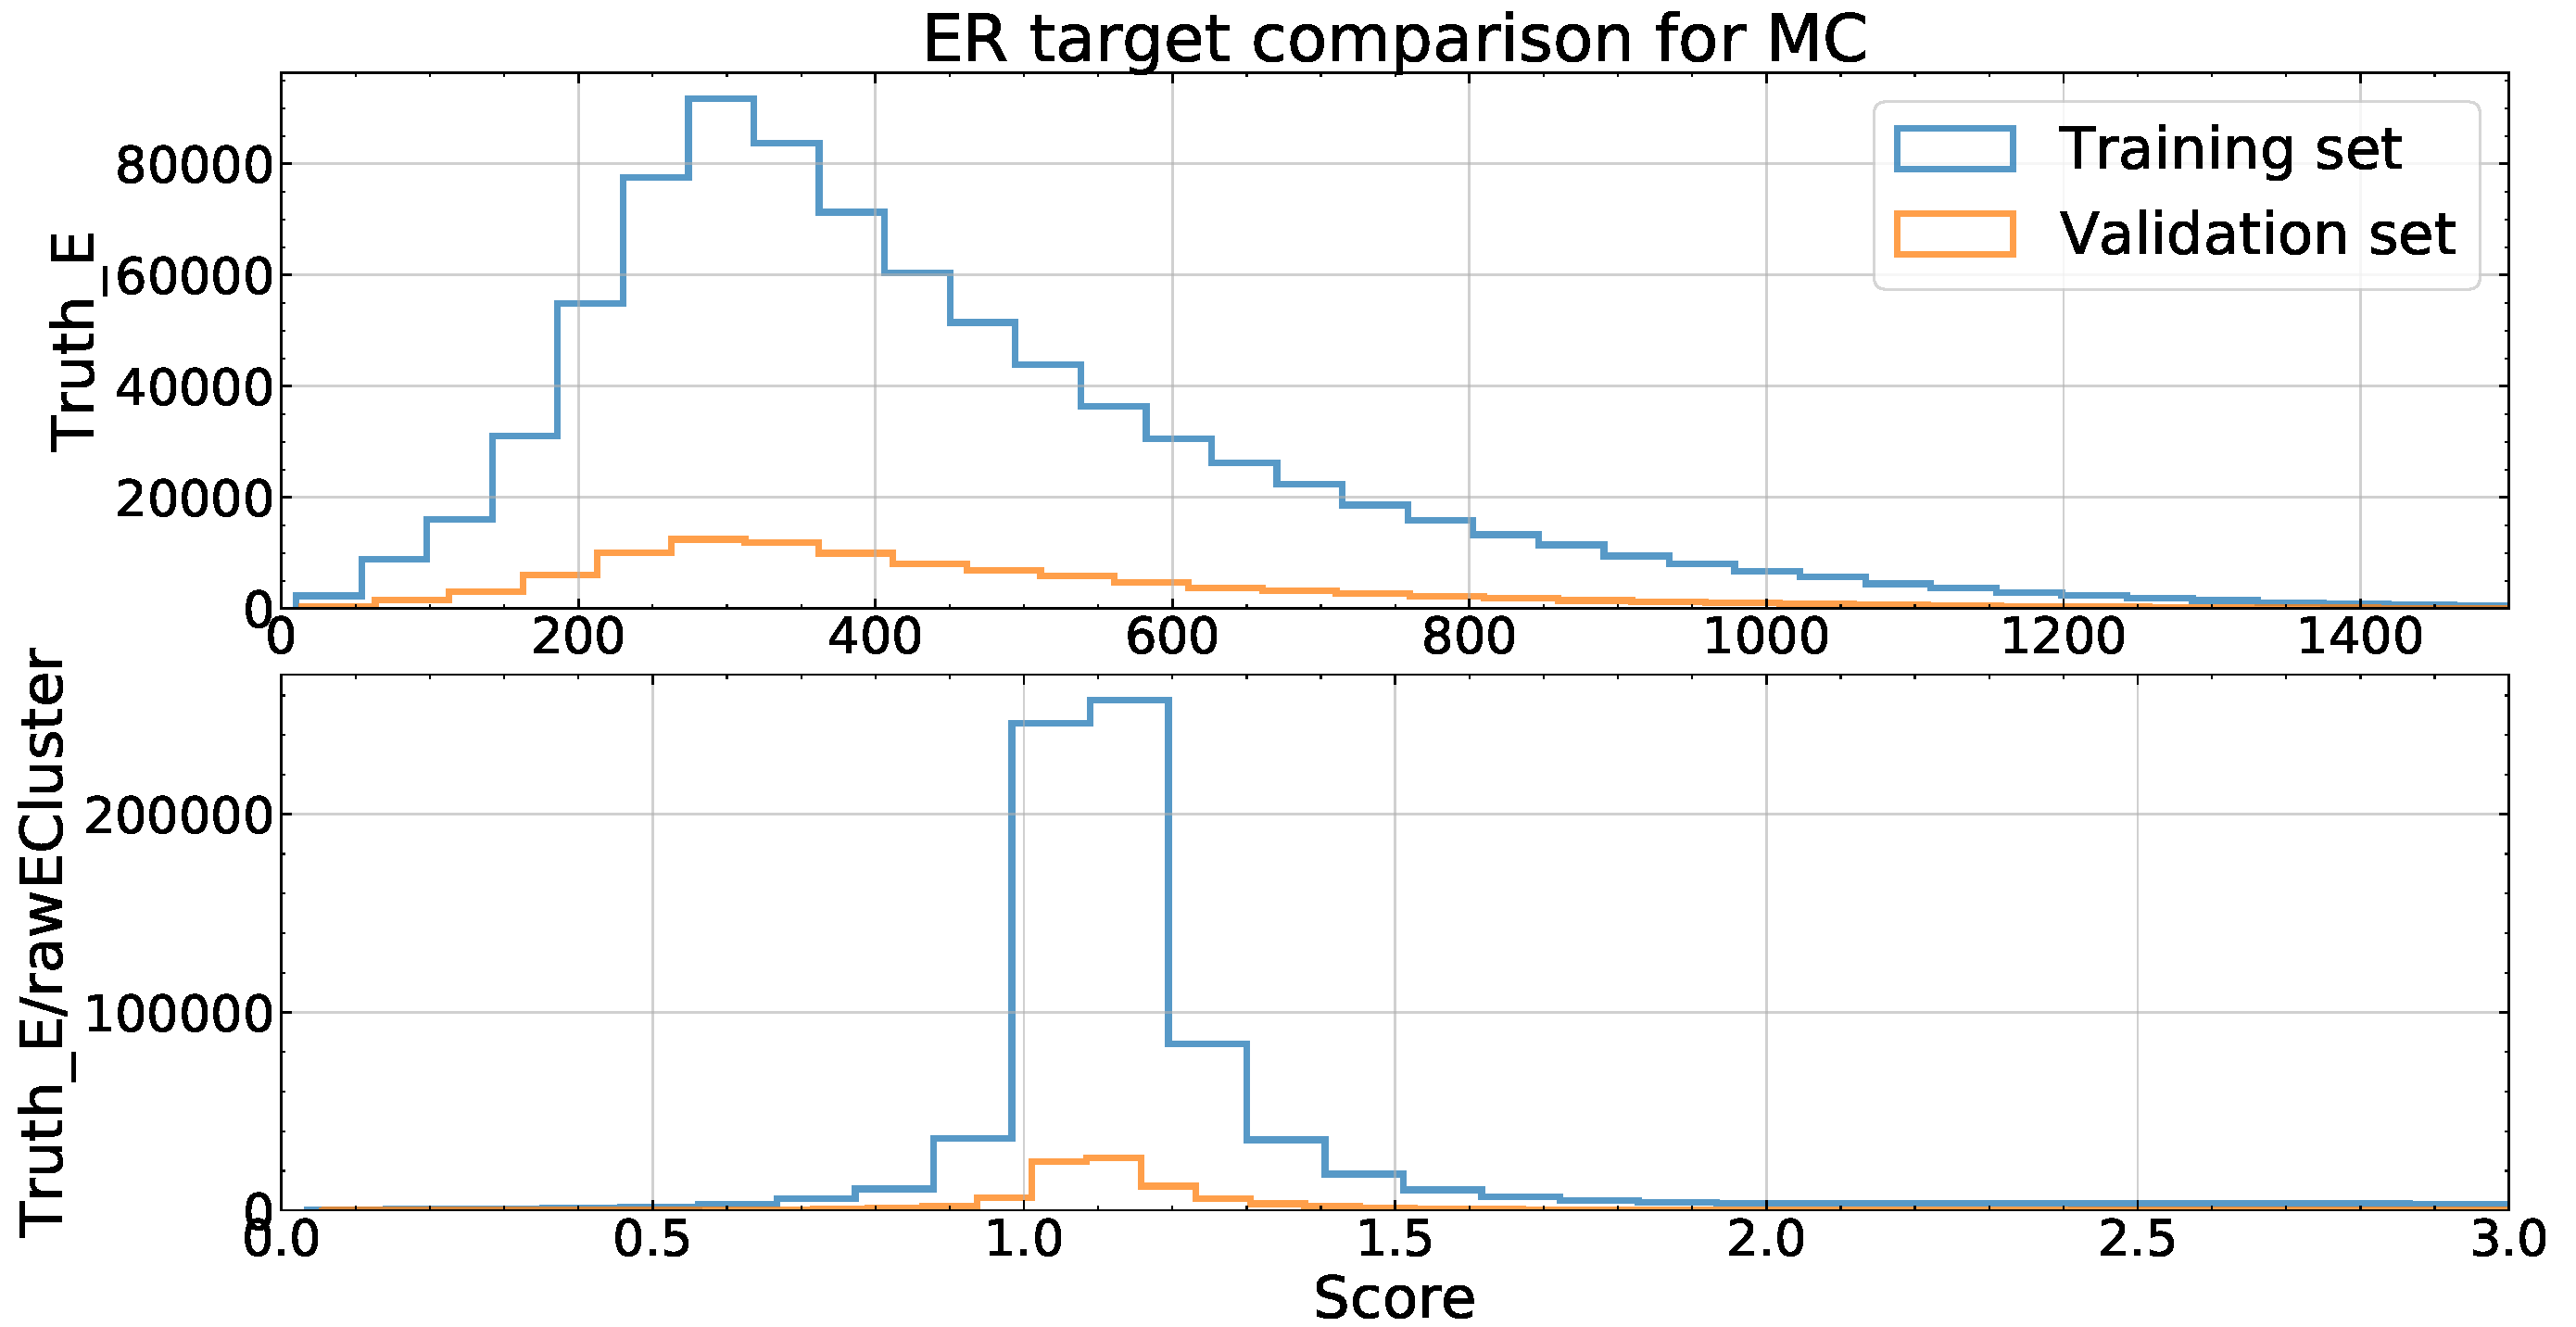
\includegraphics[width=1\linewidth]{Images/Appendix/Truth_E-v-Truth_EdivbyrawECluster.pdf}
\end{figure}
 % Appendix A
% Appendix B

\chapter{Appendix B: Production and data} \label{App:B:Prod}


\begin{table}[]
    % \addtolength{\leftskip} {-1cm}
    % \addtolength{\rightskip}{-3cm}
    \begin{tabular}{c|l}
      EGAM1 & $J \rightarrow ee$ (central) \\ \hline
      EGAM2 & $J/\psi \rightarrow ee$ \\ \hline
      EGAM3 & $Z \rightarrow ee\gamma, Z \rightarrow eee$ \\ \hline
      EGAM4 & $Z \rightarrow\mu\mu\gamma, Z \rightarrow \mu\mu e$ \\ \hline 
      EGAM5 & $W \rightarrow e\nu$ \\ \hline
      EGAM6 & \begin{tabular}[c]{@{}l@{}}$Z \rightarrow ee$\\(looser than EGAM1)\end{tabular} \\ \hline
      EGAM7 & Inclusive electrons \\ \hline
      EGAM8 & \begin{tabular}[c]{@{}l@{}}$Z \rightarrow ee$\\(At least 1 fwd $e$)\end{tabular} \\ \hline
      EGAM9 & \begin{tabular}[c]{@{}l@{}}Bootstrap for\\$\gamma$ trigger\end{tabular}
      \end{tabular}
    \marginnote{
    \caption{Overview of egamma xAOD derivations types. For more information see \citetitle{Egam_XAODderv}\citep{Egam_XAODderv}}
    \label{tab:EGAM_types}}
  \end{table}
  
 % Appendix B
% Appendix C

\chapter{Appendices} \label{App:C:Anaylsis}

Stuff % Appendix C

%----------------------------------------------------------------------------------------
%	POST-CONTENT THESIS PAGES
%----------------------------------------------------------------------------------------

\refstepcounter{dummy}
\addcontentsline{toc}{chapter}{Acronyms}
\pdfbookmark[1]{Acronyms}{acronyms}
\chapter*{Acronyms}
\begin{acronym}[UML]

\acro{AKA}{Also Known As}
\acro{ALICE}{A Large Ion Collider Experiment}
\acro{ATLAS}{A Toroidal LHC ApparatuS}
\acro{AUC}{Area Under the Curve}
\acro{BDT}{Boosted Decition Tree}
\acro{CERN}{Conseil européen pour la recherche nucléaire [English: European Organization for Nuclear Research]}
\acro{cms}{center-of-mass}
\acro{CMS}{Compact Muon Solenoid}
\acro{CSC}{Cathode Strip Chambers}
\acro{ECAL}{Electromagnetic CALorimeter}
\acro{EF}{Event Fitler}
\acro{EMEC}{ElectroMagnetic Endcap Calorimeter}
\acro{ER}{Energy Regression}
\acro{FCAL}{Forward CALorimeter}
\acro{FPR}{False Positive Rate}
\acro{GBReweighter}{Gradient Boosted Reweighter}
\acro{IBL}{Insertable B-layer}
\acro{IQR}{InterQuartile Range}
\acro{HCAL}{Hadronic CALorimeter}
\acro{HEC}{Hadronic Endcap Calorimeter}
\acro{HLT}{High Level Trigger}
\acro{L1}{Level-1 trigger}
\acro{L2}{Level-2 trigger}
\acro{LAr}{Liquid Argon}
\acro{LDA}{Linear Discriminant Analysis}
\acro{LH}{Likelihood}
\acro{HL-LHC}{High-Luminosity Large Hadron Collider}
\acro{HP}{Hyper Parameters}
\acro{ID}{Inner Detector}
\acro{LHC}{Large Hadron Collider}
\acro{LHCb}{Large Hadron Collider beauty}
\acro{MAE}{Mean Absolute Error}
\acro{MC}{Monte Carlo}
\acro{MDT}{Monitored Drift Tubes}
\acro{MET}{Missing $E_T$}
\acro{ML}{Machine Learning}
\acro{MS}{Muon Spectrometer}
\acro{MSE}{Mean Squared Error}
\acro{NN}{Neural Network}
\acro{p}{Proton}
\acro{PDF}{Probability Density Function}
\acro{PI}{Permutation Importance}
\acro{PID}{Particle IDentification}
\acro{PP}{Particle Physics}
\acro{QCD}{Quantum ChromoDynamics}
\acro{QFT}{Quantum Field Theory}
\acro{RE}{Relative Error}
\acro{RF}{Random Forest}
\acro{rIQR}{relative InterQuartile Range}
\acro{ROC}{Receiver Operating Characteristics}
\acro{RPC}{Resistive Plate Chambers}
\acro{SHAP}{SHapeley Additive exPlanations}
\acro{SCT}{SemiConductor Tracker}
\acro{SM}{Standard Model}
\acro{TGC}{Thin Gap Chambers}
\acro{TPR}{True Positive Rate}
\acro{TRT}{Transition Radiation Tracker}
\acro{VBF}{Vector-Boson Fusion}
\acro{VBS}{Vector-Boson Scattering}

\end{acronym}
\vspace{8ex}

 % Acronyms

% Colophon (a brief description of publication or production notes relevant to the edition)

% \pagestyle{empty}

% \hfill

% \vfill

% \pdfbookmark[0]{Colophon}{colophon}

% \section*{Colophon}

% This document was typeset using the typographical look-and-feel \texttt{classicthesis} developed by Andr\'e Miede. The style was inspired by Robert Bringhurst's seminal book on typography ``\emph{The Elements of Typographic Style}''. \texttt{classicthesis} is available for both \LaTeX\ and \mLyX: 

% \begin{center}
% \url{https://bitbucket.org/amiede/classicthesis/}
% \end{center}

% \noindent Happy users of \texttt{classicthesis} usually send a real postcard to the author, a collection of postcards received so far is featured here: 

% \begin{center}
% \url{http://postcards.miede.de/}
% \end{center}
 
% \bigskip

% \noindent\finalVersionString

\refstepcounter{dummy}
\addcontentsline{toc}{chapter}{\listfigurename} % Uncomment if you would like the list of figures to appear in the table of contents
\pdfbookmark[1]{\listfigurename}{lof} % Bookmark name visible in a PDF viewer

\listoffigures

\vspace{8ex}
 % List of figures - updates automatically

% Declaration

% \refstepcounter{dummy}
% \pdfbookmark[0]{Declaration}{declaration} % Bookmark name visible in a PDF viewer

% \chapter*{Declaration} % Declaration section text

% \thispagestyle{empty}

% Put your declaration here.
% \bigskip
 
% \noindent\textit{\myLocation, \myTime}

% \smallskip

% \begin{flushright}
% \begin{tabular}{m{5cm}}
% \\ \hline
% \centering\myName \\
% \end{tabular}
% \end{flushright}

\refstepcounter{dummy}
\addcontentsline{toc}{chapter}{\listtablename} % Uncomment if you would like the list of tables to appear in the table of contents
\pdfbookmark[1]{\listtablename}{lot} % Bookmark name visible in a PDF viewer

\listoftables
        
\vspace{8ex}

 % List of Tables - updates automatically

% Bibliography

\label{app:bibliography} % Reference the bibliography elsewhere with \autoref{app:bibliography}

\manualmark % Work-around to have small caps also here in the headline
\markboth{\spacedlowsmallcaps{\bibname}}{\spacedlowsmallcaps{\bibname}} % Work-around to have small caps also
%\phantomsection
\refstepcounter{dummy}
 
\addtocontents{toc}{\protect\vspace{\beforebibskip}} % Place the bibliography slightly below the rest of the document content in the table of contents
\addcontentsline{toc}{chapter}{\tocEntry{\bibname}}

\printbibliography % Bibliography


\cleardoublepage
%----------------------------------------------------------------------------------------

\end{document}
